\section{Vorwort}
Bei der Recherche zur Bearbeitung der Übungen wurden viele englischsprachige Webseiten zu rate gezogen. Generell kann man sagen, dass englische Fachbegriffe sich im Bereich FPGA und embedded Design etabliert haben, so dass eine Übersetzung eher verwirren als helfen würde. Daher haben wir uns entschieden, die \textbf{englischen} Bezeichner und Beschreibungen beizubehalten.\\
Um Codeabschnitte besser von Beschreibungen besser unterscheiden zu können, wurde eine eigene Schriftart verwendet:
\begin{verbatim}
  Kommandozeilen Eingaben und Codesnippets werden wie HIER dargestellt.
\end{verbatim}


\section{Projektbeschreibung 1} \label{ex1}
Info...


\subsection {Die Zahl ...}
weitere Unterpunkte

\subsection {Eine ...}
Da es sich bei den D


Beispielbild....

\begin{minipage}{\textwidth}
    \begin{center}        
        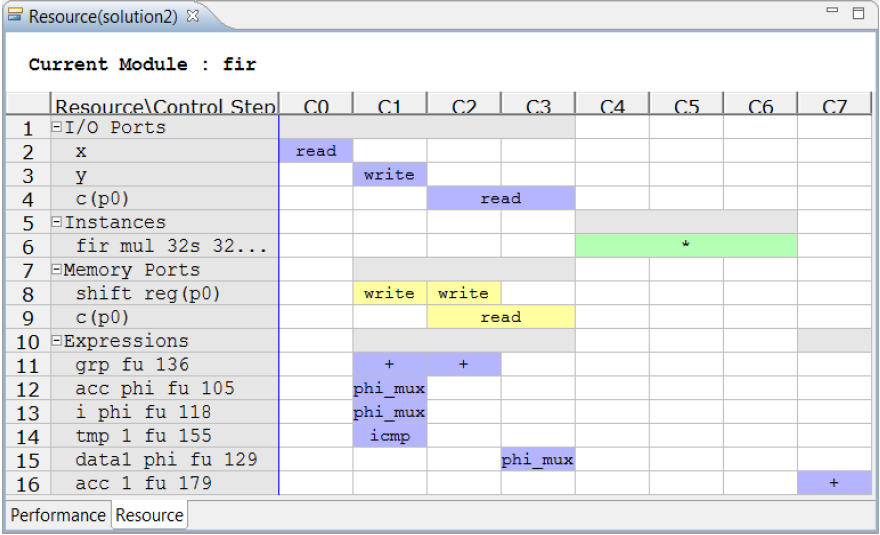
\includegraphics[scale=0.7]{img/Resource.png} 
    \end{center}
\end{minipage}
\begin{center}
Multiplikationsformel
\end{center}

\subsection {die benötigten Operationen des Design und deren Laufzeit}
In der linken Feld der Performance\-Ansicht werden die Operationen im Modul der RTL\-Hierarchie angezeigt.\\


